\section{Einleitung}

Der heutige Netzwerkverkehr ist fast tausendfach größer als vor 20 Jahre \citep{Roser_I}. Das Internet wird heutzutage für fast alle unsere alltägliche Tätigkeit verwendet: Soziale Netzwerke, Video und Audio-Streaming, Einkauf, behördliche Angelegenheit und viele andere. So viel Verkehr generiert eine unermessliche Menge von Daten, die alle mögliche Inhalte beinhalten, von unschuldigen Anfragen nach dem eigenen Kontostand bis zu der Ausführung von bösewichten Anfragen, um Systemen lahmzumachen. Um das erste von der zweiten zu unterscheiden verwenden viele Firmen das sogenannte \glsfirst*{SIEM} oder Log Analysis Tools.

Das \glsfirst{NIST} definiert \acrshort{SIEM} als Software für die Sammlug, Anpassung, Analyse, Überwachung und Bedrohungserkennung von Sicherheitsdaten aus verschiedenen Quellen, damit das zuständige \glsfirst{SOC} Maßnahmen ergreifen kann \citep{NIST_Definitions}. Die Bewertung dieser Daten spielt eine wesentliche Rolle bei solchen Anwendungen, da es entscheidend ist, zu wissen, ob es sich um normale Anfrage oder um \glsplural{Cyberangriff} handelt. Log Analysis und Log Management beziehen sich auf die Sammlung, Bearbeitung, Speicherung und/or Löchen, Weiterleitung und Überwachung von Loginformationen. In dieser Arbeit benutzen wir den Begriff \quotes{Log Analysis Tool}, um diese Systemen zu referenzieren

In diesem Projekt recherchieren und vergleichen wir  existierende \gls{SIEM} und Log Analysis Tools. Danach entscheiden wir uns für eine \gls{Open Source} Lösung, sodass wir sie für spezifische Logdateien der Hochschule Worms anwenden können. Die Angriffserkennung soll automatisch mit der Eingabe von vordefinierten Regeln der \gls{mitre} Matrix stattfinden.

Diese Arbeit wird in folgende Teile geteilt:

% OSSIN: https://sourceforge.net/projects/os-sim/
% Preludes: https://www.prelude-siem.org/projects/prelude/wiki/ManualUser
% ELK Stack

% Grafana / Promtail: https://grafana.com/products/enterprise/
%https://grafana.com/logs/% 

%https://www.ossec.net/         https://github.com/ossec/ossec-rules

% was machen sie konkrent? / Vergleich zwischen OpenSource/Proprietary/

\begin{itemize}[noitemsep]
   \item Definition von \glspl{SIEM} und Log Analysis Tools
   \item Beschreibung von existierenden \gls{Proprietary} und \gls{Open Source} Lösungen
   \item Entscheidung für die Implementation einer \gls{Open Source} Lösungen
   \item Installation und Konfiguration von der ausgewählten Anwendung 
   \item Definition von zwei spezifischen \glsplural{Cyberangriff}
   \item Festelung von Regeln oder \gls{usecases} für die automatische Erkennenung von der vorherigen definierten Angriffe Anhand der \gls{mitre} Matrix
   \item Empfang, Bearbeitung und Eingabe in der ausgewählten Lösung der spezifischen Logdatein der Hochschule
   \item Analyse, Bewertung und Zukunft dieser Recherche
\end{itemize}

Das folgende Diagramm stellt den Aufbau dieser Arbeit dar:

% Diagram anpassen mit korrenkten Zielen

\begin{figure}[H]
   \centering
   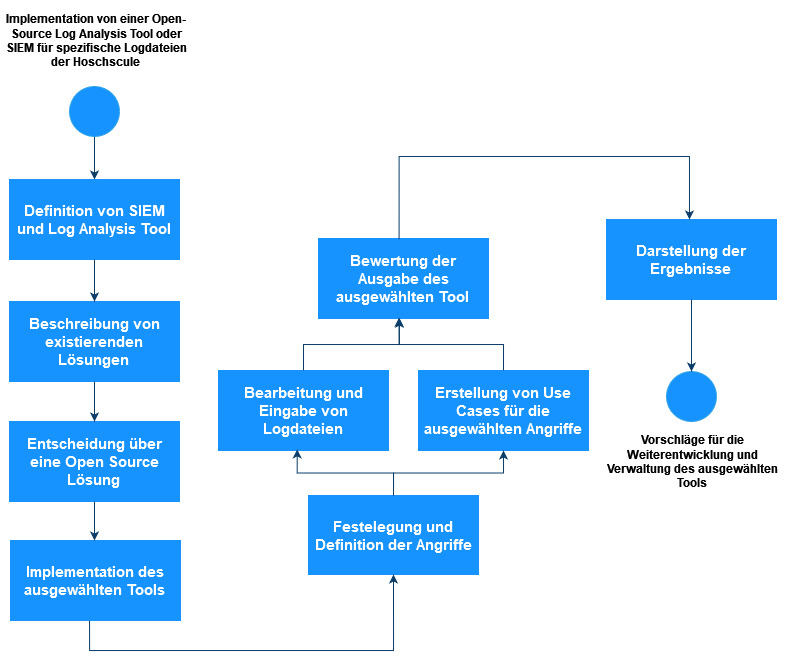
\includegraphics[width=1\textwidth]{assets/1_p1.jpg}
   \caption{Aufbau dieser wissenschaftlichen Recherche \gls{SIEM} \\Quelle: Eigene Darstellung }
   \centering
\end{figure}

\subsection{Problemstellung}
Während der Entwicklung dieser Arbeit wollen wir uns mit folgenden Fragen beschäftigen:

% Regeln anhand mittre, automatisieren
\begin{itemize}
   \item Wie können wir ein Log Analysis Tool so konfigurieren, dass es vordefinierten Angriffe nach der \gls{mitre} Matrix automatisch erkennen kann?
   \item Wie können wir eine allgemeine \gls{usecases} definieren, sodass wir sie später für verschiedene Angriffsmuster nach \gls{mitre} Matrix leicht anpassen können?
\end{itemize}

\textcolor{red}{\textbf{Note: Für Angriffe habe ich an DoS und Brute-Force (Password Spraying/Dictionary) gedacht.}}


\subsection{Vorgehensweise}
Um diese oben genannten Ziele zu erreichen, verwenden wir folgenden Methode:

\begin{itemize}[noitemsep]
   \item Recherche in der Fachliteratur über \glsplural{SIEM} und Log Analysis Tools Lösungen
   \item Vergleich zwischen verschiedenen \gls{Open Source} und \gls{Proprietary} Lösungen
   \item Installation von der ausgewählten Tool  
   \item Importieren von Logdateien in der ausgewählten \gls{SIEM} Lösung
   \item Definition der \gls{usecases} für die Angriffe
\end{itemize}

